\documentclass[letterpaper,journal]{IEEEtran}
\usepackage{amsmath,amssymb,amsfonts}
\usepackage{booktabs}
\usepackage{graphicx}
\usepackage{cite}
\usepackage{url}
\usepackage[hidelinks]{hyperref}
\usepackage{xcolor}

\newcommand{\Tr}{\operatorname{Tr}}
\newcommand{\E}{\mathbb{E}}
\newcommand{\A}{\mathcal A}
\newcommand{\T}{\mathcal T}
\newcommand{\C}{\mathbb C}
\newcommand{\SAOC}{\textsc{SAOC}}

\begin{document}

\title{Symmetry-Resolved Observable Contrast: Exact Invariant Witnesses and Data-Driven Order Parameters}

\author{Rongzhou (Lachlan) Chen%
\thanks{Working paper. All numerical claims are backed by fixed-seed scripts,
raw records, and manifests in the accompanying public repository. Chemistry
and robotics results are controlled models, not deployment claims.}}

\maketitle

\begin{abstract}
The most discriminative observable may be physically inaccessible: it can
depend on an arbitrary origin, violate a symmetry, or require an unrealizable
instrument. We solve maximum observable contrast inside a
finite-dimensional accessible observable algebra. If
$\mathcal E_{\mathcal A}$ is the trace-preserving conditional expectation
onto a unital $*$-subalgebra $\mathcal A$, the largest expectation gap over
effects in $\mathcal A$ is the trace of the positive part of
$\mathcal E_{\mathcal A}(\rho_1-\rho_0)$. Compact-group symmetry is the
special case of twirling onto the commutant. Representation blocks then
decompose distinguishability into physical sectors, while cyclic translation
reduces exactly to Fourier power and admits $O(d\log d)$ updates. Controlled
experiments verify the consequences. With only two training signals per
class, translation-invariant contrast obtains $99.986\%$ accuracy versus
$50\%$ for untwirled contrast and raw linear classification; a correctly
specified Fourier-power classifier is perfect, isolating the value of the
symmetry prior. A ten-qubit transverse-field Ising reduced-state response
peaks at $g/J=0.9625$, near the thermodynamic critical point 1, and resolves
parity sectors. A H{\"u}ckel difference density yields balanced attachment and
detachment modes to $5.6\times10^{-17}$, and a simulated six-axis contact
witness has $0.9993$ overlap with the planted wrench screw. The framework
unifies invariant testing, spectral diagnostics, optics, and density
differences. Connections to gauge theory, quantum field theory, and
holography are stated as concrete future calculations, not as a string-theory
solution.
\end{abstract}

\begin{IEEEkeywords}
group invariance, interpretable physics, quantum state discrimination,
symmetry-resolved analysis, trace distance
\end{IEEEkeywords}

\section{Introduction}

\IEEEPARstart{A}{n} unconstrained detector answers the wrong question when the
observer has no absolute phase, the material is translation invariant, or
only gauge-invariant readouts are physical. Data augmentation can approximate
invariance, but it does not by itself identify the best realizable measurement
or quantify which symmetry sector changed.

Invariant quantum hypothesis testing is established
theory~\cite{hiai2009}, and harmonic analysis provides the associated
representation blocks~\cite{serre1977,marvian2014}. Symmetry-resolved
entanglement likewise decomposes reduced states into charge
sectors~\cite{goldstein2018}. We combine these ideas with additive
positive-state summaries to construct symmetry-/subalgebra-accessible
observable contrast (\SAOC). The central result is deliberately more general
than a group: locality, block readout, bandwidth, and coarse graining can all
be encoded as an accessible operator algebra.

This paper contributes:

\begin{enumerate}
\item a finite-dimensional conditional-expectation theorem for the optimal
accessible bounded effect and its compact-group corollary;
\item a sector decomposition that turns a scalar detector into a physical
diagnostic, plus an exact fast Fourier case;
\item reproducible tests in signals, many-body physics, one-electron
chemistry, and robot contact, including matched baselines and explicit
negative boundaries;
\item a precise route toward gauge-invariant reduced-state comparison in
quantum field and string-theoretic models without claiming such a calculation
has already been completed.
\end{enumerate}

\section{Accessible-Observable Theory}

\subsection{Unrestricted contrast}

Let $\rho_0,\rho_1\succeq0$ have unit trace and
$\Delta=\rho_1-\rho_0$. Over all effects $0\preceq E\preceq I$,
\begin{equation}
\max_E\Tr(E\Delta)=\Tr(\Delta_+)=\tfrac12\|\Delta\|_1, \label{eq:helstrom}
\end{equation}
with $E^\star=\mathbf1_{\Delta>0}$. This is the operational trace-distance
result of binary quantum discrimination~\cite{helstrom1976}. We ask what
remains when $E$ must belong to the physical readout algebra.

\subsection{Conditional expectation theorem}

Let $\A\subseteq M_d(\C)$ be a unital $*$-subalgebra, and let
$\mathcal E_\A:M_d\rightarrow\A$ be the trace-preserving conditional
expectation (the Hilbert--Schmidt orthogonal projection onto $\A$).

\textbf{Theorem 1 (accessible contrast).}
\begin{equation}
\sup_{\substack{E\in\A\\0\preceq E\preceq I}}\Tr(E\Delta)
=\Tr\!\left[\mathcal E_\A(\Delta)_+\right].          \label{eq:algebra}
\end{equation}
An optimizer is the positive support projector of
$\mathcal E_\A(\Delta)$, formed inside $\A$.

\begin{IEEEproof}
For $E\in\A$, orthogonal projection gives
$\Tr(E\Delta)=\Tr[E\mathcal E_\A(\Delta)]$.
Conditional expectation preserves Hermiticity and
$\mathcal E_\A(\Delta)\in\A$. Applying the Jordan bound within the
finite-dimensional algebra proves the upper bound. Functional calculus in a
$*$-algebra places the positive support projector in $\A$, so the bound is
attained.
\end{IEEEproof}

The accessible distance is no larger than the unrestricted distance:
coarse graining cannot increase distinguishability. Equality holds exactly
when an unrestricted optimal effect has an equivalent representative in
$\A$. This supplies a falsifiable measure of how much information an
instrument constraint discards.

\subsection{Group symmetry and sectors}

For a compact group with unitary representation $U_g$, the commutant
$\A=\{U_g\}'$ contains invariant observables. Its conditional expectation is
the twirl
\begin{equation}
\T_G(X)=\int_GU_gXU_g^\dagger\,dg.                  \label{eq:twirl}
\end{equation}
Thus,
\begin{equation}
\max_{\substack{0\preceq E\preceq I\\{}[E,U_g]=0}}
\Tr(E\Delta)=\Tr[\T_G(\Delta)_+].                   \label{eq:symopt}
\end{equation}
This one-shot finite-dimensional identity is consistent with the broader
asymptotic study of symmetry-constrained quantum testing~\cite{hiai2009}.

If
\begin{equation}
\mathcal H=\bigoplus_\lambda V_\lambda\otimes M_\lambda,
\end{equation}
Schur's lemma gives
\begin{equation}
\T_G(\Delta)=
\bigoplus_\lambda
\frac{I_{V_\lambda}}{\dim V_\lambda}\otimes\Delta_\lambda. \label{eq:block}
\end{equation}
Trace norm and positive gap add over $\lambda$. Each block is therefore a
charge, parity, frequency, angular-momentum, or other representation-sector
contribution, rather than an unnamed latent feature.

\subsection{Cyclic translations}

For the regular representation of $C_d$, the DFT diagonalizes every invariant
operator. For a normalized signal $x$,
\begin{equation}
\T_{C_d}(|x\rangle\langle x|)
=F^\dagger\operatorname{diag}(|Fx|^2)F.             \label{eq:power}
\end{equation}
The class state is the mean normalized power spectrum, and the optimal
invariant effect selects positive spectral-contrast bins. Accumulation uses
an FFT and a vector addition, $O(d\log d)$ time and $O(d)$ state, rather than
a dense $d\times d$ matrix.

\section{Experimental Design}

Every output has raw CSV, a JSON summary, a deterministic command, package
versions, a Git identifier, and SHA-256 hashes. Unit tests compare FFT and
explicit group twirls, invariant analytic and SDP optima, sector additivity,
trace-distance contraction, Ising parity commutation, and H{\"u}ckel density
normalization.

\subsection{Translation nuisance}

The two classes are length-128 sinusoids at DFT bins 5 and 17. Every signal
has random cyclic shift, random phase, Gaussian noise $0.8$, and an exact
negative partner. We vary training pairs per class from 1 to 16 and test on
600 signals per class over 12 seeds. Compared methods are raw linear
logistic, untwirled rank-two contrast, invariant rank-two contrast, and a
logistic classifier on the full Fourier-power representation.

\begin{figure}[t]
\centering
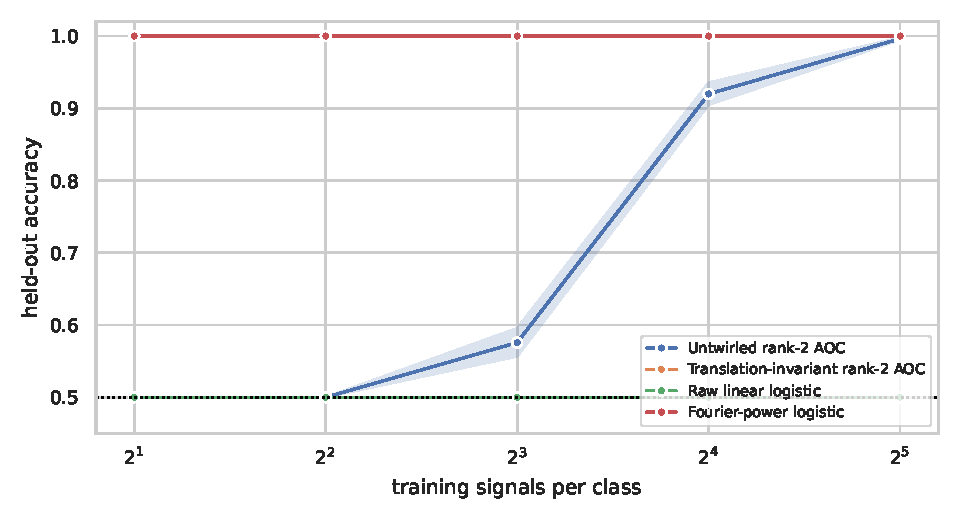
\includegraphics[width=\columnwidth]{../../experiments/run3/results/translation/translation_sample_efficiency.pdf}
\caption{Translation-nuisance sample efficiency. The invariant method and
the correctly engineered Fourier baseline solve the task immediately; raw
methods require enough shifts to estimate the orbit and linear means remain
blind.}
\label{fig:translation}
\end{figure}

\subsection{Quantum phase response}

We exactly diagonalize a periodic ten-qubit transverse-field Ising chain,
\begin{equation}
H=-\sum_iZ_iZ_{i+1}-g\sum_iX_i,
\end{equation}
trace out five qubits, and compare adjacent reduced states on a field grid
$\delta g=0.025$. The subsystem parity $X^{\otimes5}$ defines even and odd
sectors. Trace-distance diagnostics are established tools for many-body
states~\cite{zhang2019,khasseh2023}; the purpose here is sector-resolved
witness validation, not discovery of an unknown model.

\begin{figure}[t]
\centering
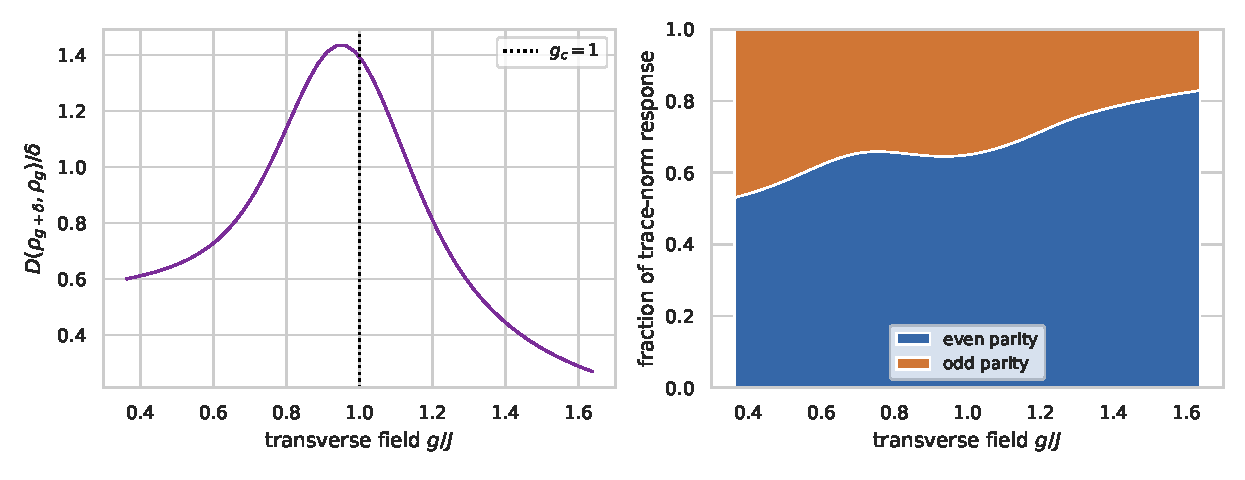
\includegraphics[width=\columnwidth]{../../experiments/run3/results/quantum_phase/symmetry_resolved_transition.pdf}
\caption{Reduced-state trace-distance response and parity-sector
decomposition in the ten-qubit transverse-field Ising model. The dotted line
is the thermodynamic critical field.}
\label{fig:quantum}
\end{figure}

\subsection{Difference-density chemistry}

A half-filled ten-site H{\"u}ckel ring is changed from uniform hopping to
alternating hopping $1\pm\delta$. The normalized occupied one-particle
projectors are twirled over two-site translations. Positive and negative
eigenvectors of their difference are natural attachment and detachment
orbitals, an interpretation already used in molecular
analysis~\cite{yamaki2015,bovill2026}. The example is a conservation and
interpretability check, not predictive electronic structure.

\subsection{Robot contact}

A six-axis force/torque residual has zero mean. Contact adds a rank-one
covariance along the physically valid wrench screw
$s\propto[n^\top,(r\times n)^\top]^\top$. Exact sign pairing eliminates mean
information. We learn a rank-one effect and compare it with the planted screw
and window-mean logistic regression across window lengths 1, 4, 16, and 64,
12 seeds each. This is a structured simulation pending hardware or public
dataset validation.

\begin{figure}[t]
\centering
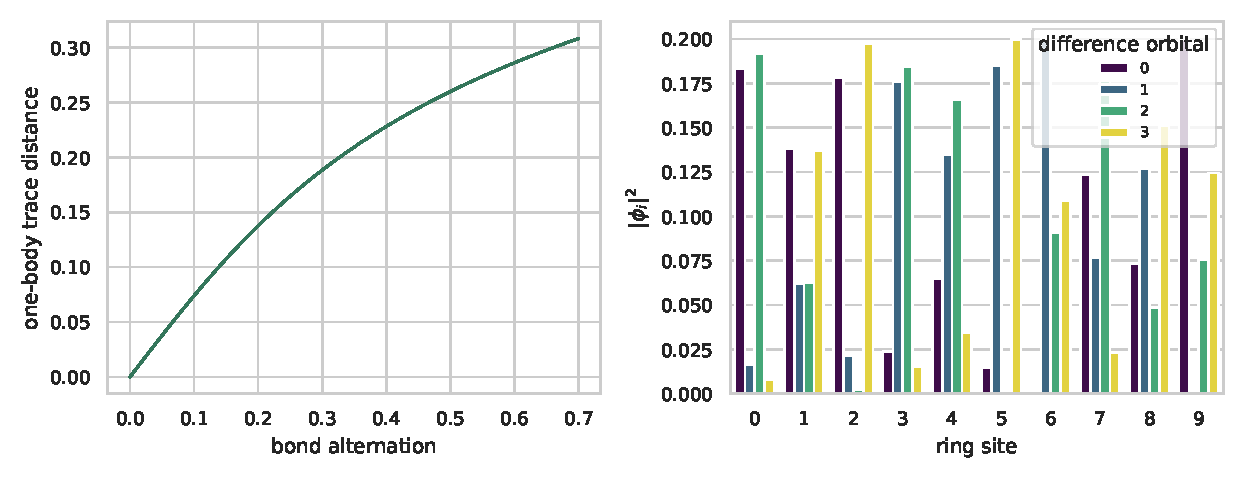
\includegraphics[width=\columnwidth]{../../experiments/run3/results/chemistry/huckel_difference_density.pdf}
\caption{Controlled H{\"u}ckel result: total one-body state change and leading
natural difference orbitals at maximum bond alternation.}
\label{fig:chem}
\end{figure}

\begin{figure}[t]
\centering
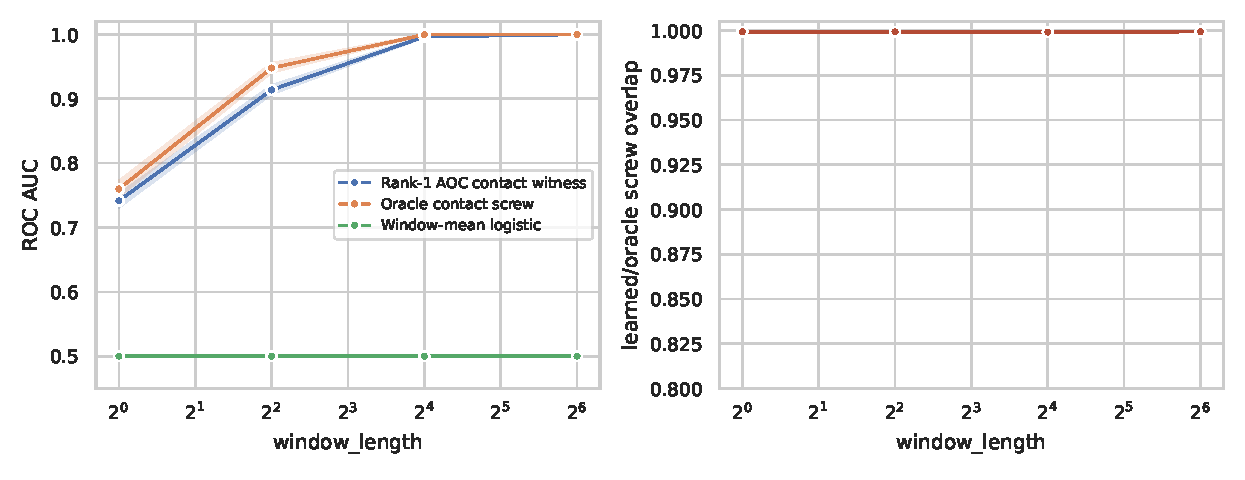
\includegraphics[width=\columnwidth]{../../experiments/run3/results/robot_contact/robot_contact_detection.pdf}
\caption{Controlled robot-contact result. A low-rank quadratic witness
recovers the planted wrench direction while the sign-paired mean is blind.}
\label{fig:robot}
\end{figure}

\section{Results}

At two training signals per class, Fig.~\ref{fig:translation} gives mean
accuracy $0.999861$ for invariant contrast, $1.0$ for Fourier-power logistic,
and exactly $0.5$ for raw logistic and untwirled contrast. This is not evidence
that \SAOC\ beats an appropriate invariant feature map: they tie. It shows
that quotienting an exactly known nuisance can transform the small-sample
problem, while a learned orbit average needs more examples.

The trace-distance susceptibility in Fig.~\ref{fig:quantum} peaks at
$g/J=0.9625$, close to the exact thermodynamic value 1. The maximum parity
commutator residual is $3.54\times10^{-9}$. Finite-size displacement is
expected; no critical exponent is inferred from one size. The result
demonstrates that the learned bounded witness and its sector weights can serve
as a data-driven response diagnostic alongside conventional order
parameters~\cite{carrasquilla2017}.

At bond alternation $0.7$, Fig.~\ref{fig:chem} gives one-body trace distance
$0.30845$. Positive attachment and negative detachment weights balance to
$5.55\times10^{-17}$, as required by particle-number conservation. In real
atom-centered nonorthogonal bases, the overlap metric and correlated density
construction must be handled explicitly.

At 64-sample windows, both the learned and oracle contact scores in
Fig.~\ref{fig:robot} have ROC AUC $1.0$, whereas mean logistic has $0.5$ by
construction. Learned/oracle screw overlap averages $0.99925$. The correct
conclusion is recovery in a matched rank-one model, not robustness to payload,
pose, friction, or sensor drift.

\section{Connections and Boundaries}

\subsection{Optics, vision, and atomistic representations}

Normalized optical coherency matrices are density operators, so an accessible
algebra can encode available wave plates, apertures, polarization analyzers,
or spatial modes~\cite{mandelwolf1995}. In vision and vibration, translation
twirling gives an exact phase-blind power detector. It cannot distinguish
homometric or phase-coded signals; bispectra, higher tensor states, or
equivariant models are then necessary.

For molecular environments, rotations lead to spherical-harmonic blocks.
SOAP~\cite{bartok2013} and the atomic cluster
expansion~\cite{drautz2019} already provide systematic invariant
representations. A credible use of \SAOC\ is supervised, streaming selection
of discriminative blocks from those established features, not replacement
without molecular benchmarks.

\subsection{Quantum field theory and string theory}

The connection is a research program, not a solved application. Reduced states
in quantum field theory can be compared by trace distance~\cite{zhang2019},
and symmetry-resolved entanglement assigns contributions to conserved-charge
blocks~\cite{goldstein2018}. Given two computable reduced states
$\rho_A(\theta)$ and $\rho_A(\theta+\delta)$, \SAOC\ asks which bounded,
gauge-invariant regional observable best distinguishes the couplings or
backgrounds.

This question can be posed in lattice gauge theory, tensor networks, conformal
field theory, and holography. The Ryu--Takayanagi relation connects boundary
entanglement to bulk geometry~\cite{ryu2006}, while the entanglement first law
and modular Hamiltonian enter gravitational dynamics~\cite{lashkari2014}.
They are not identical to \SAOC: a modular Hamiltonian
$K=-\log\rho$ is a distinguished, generally unbounded state-dependent
observable, whereas \SAOC\ optimizes a bounded operational effect. Comparing
their responses is meaningful; equating them without proof is not.

Gauge theories also need care because spatial Hilbert-space factorization and
edge modes depend on the chosen observable algebra. A falsifiable first
project is a small published lattice-gauge or matrix-product-state model:
predeclare two couplings, form gauge-invariant reduced states, compute sector
witnesses, and compare them with known flux or Wilson-loop diagnostics. Until
that calculation exists, the repository makes no claim about a new string
vacuum, duality, or quantum-gravity solution.

\subsection{Failure modes}

Twirling deliberately deletes asymmetry. If orientation or phase is the
signal, invariant contrast is worse than the unrestricted method. Sector
weights can be stable while eigenvectors inside a degenerate block are not
identifiable. Dense non-Abelian decompositions can be expensive, and
empirical state error can dominate small sector gaps. Physical instruments
may impose a convex set that is not a $*$-algebra; then
Eq.~\eqref{eq:algebra} is replaced by a general convex optimization.

\section{Conclusion}

Maximum observable contrast becomes physically meaningful only after the
accessible measurements are specified. Conditional expectation projects the
state difference onto that algebra; the positive part gives the exact optimal
effect; and symmetry blocks reveal where distinguishability resides. The
fast translation case, many-body parity response, difference-density
orbitals, and contact wrench recovery show one operator principle across
domains while preserving honest baselines. The strongest next tests are
real streaming instruments and a concrete gauge-invariant many-body
calculation.

\bibliographystyle{unsrt}
\bibliography{references}

\end{document}
